\documentclass[
11pt,%
tightenlines,%
twoside,%
onecolumn,%
nofloats,%
nobibnotes,%
nofootinbib,%
superscriptaddress,%
noshowpacs,%
centertags]%
{revtex4}
\usepackage{ljm}
\usepackage{listings}

\lstset{
language=C++,
basewidth=0.5em,
xleftmargin=45pt,
xrightmargin=45pt,
basicstyle=\small\ttfamily,
keywordstyle=\bfseries\underbar,
numbers=left,
numberstyle=\tiny,
stepnumber=1,
numbersep=10pt,
showspaces=false,
showstringspaces=false,
showtabs=false,
frame=trBL,
tabsize=2,
captionpos=t,
breaklines=true,
breakatwhitespace=false,
escapeinside={\%*}{*)}
}

\begin{document}

\titlerunning{Process Mining}
\authorrunning{Savin et al.}

\title{Process Mining: Realization and Optimization of Process Discovery Algorithm}

\author{\firstname{G.~I.}~\surname{Savin}}
\email[E-mail: ]{savin@jscc.ru}
\affiliation{Joint Supercomputer Center of the Russian Academy of Sciences -- branch of Scientific Research Institute of System Analysis of the Russian Academy of Sciences, Leninsky prospect 32a, Moscow, 119334, Russia}

\author{\firstname{A.~D.}~\surname{Chopornyak}}
\email[E-mail: ]{chopor@jscc.ru}
\affiliation{Joint Supercomputer Center of the Russian Academy of Sciences -- branch of Scientific Research Institute of System Analysis of the Russian Academy of Sciences, Leninsky prospect 32a, Moscow, 119334, Russia}

\author{\firstname{A.~A.}~\surname{Rybakov}}
\email[E-mail: ]{rybakov.aax@gmail.com}
\affiliation{Joint Supercomputer Center of the Russian Academy of Sciences -- branch of Scientific Research Institute of System Analysis of the Russian Academy of Sciences, Leninsky prospect 32a, Moscow, 119334, Russia}

\author{\firstname{S.~S.}~\surname{Shumilin}}
\email[E-mail: ]{shumilin@jscc.com}
\affiliation{Joint Supercomputer Center of the Russian Academy of Sciences -- branch of Scientific Research Institute of System Analysis of the Russian Academy of Sciences, Leninsky prospect 32a, Moscow, 119334, Russia}

\firstcollaboration{(Submitted by S.~S.~Submitter)}

\received{May 01, 2020}

\begin{abstract}
Abstract.
\end{abstract}

\subclass{68R10} % Enter 2010 Mathematics Subject Classification.

\keywords{Process mining, process discovery algorithm, Petri nets, process model, event logs.}

\maketitle

\section{Introduction}

Process mining is a collection of approaches and methods for extracting process related information from event logs.
Process mining is closely related to areas such as business process management (BPM) and workflow management (WFM).
WFM technology has historically been primarily aimed at automating business processes from a mechanical point of view, while using BPM approaches, special attention is paid to other aspects in which bottlenecks can be hidden (human factor, organization features, fuzzy rules, and others).
Currently, many process-aware information systems (PAIS), in addition to the classic WFM tools, include BPM extensions and process mining approaches.
However, often these systems remain analysis and notification systems, being insufficiently integrated into the digital space.
Along with the term PAIS, the term BPMS (BPM system) or simply PMS (process management system) is also used for such systems.

Any process analysis system works with a process model that is written using one or more notations.
These notations represent the essence of the process and are essentially macro-descriptions of oriented graphs of a special kind.
The main objects of process models are activities, states, transitions and subprocesses.
Transitions between different activities are also called dependencies.
The set of dependencies between activities and also additional conditions imposed on the process model give rise to many possible sequences of state changes, or many scenarios of the process.
Depending on the details of the processes, additional attributes of any objects of the process model can be used: time references, duration of activities, dependency logic, resources and strategies for their use, roles of activity performers, and many others.
Such a variety that arises in the modeling of processes generates a huge number of methods for analyzing processes and scenarios, and can serve as a source of useful and not always obvious knowledge used to optimize processes.

Process models recorded using formal notation can be used for various purposes: a review from various points of view, discussion of a process model between all participants, preparation of documentation (including in automatic mode), verification (some obvious errors may be detected just by analyzing the topology of the model graph, for example, it can be dead sections of the process, deadlocks, infinite loops and others), performance analysis (using simulations on the process model can be bottlenecks identified and eliminated), visualization of the process to simplify the analysis, specification (from the formal model, descriptions of interfaces and interaction protocols can be generated even before integration into a single digital space), configuration (the description of the process model can be used to configure the system when its implementation).
Typically, when developing a process, there is both an informal model (used for discussion and documentation) and a formal model suitable for simulations (used for analysis and improvement). 

Informal models are often divorced from life, abstract, idealized, while formal models, on the contrary, are too detailed and often understandable only to the actual developers of the model.
There is no middle ground between these two models, and this often leads to additional risks when developing a process model, since in fact the tested and analyzed executable model is very different from the model at the presentations.
But even this is not the main problem.

The main problem of any process model is that it is not known in advance how much the model relates to reality.
In reality, people are included in the processes, the logic of their interaction with the system is immeasurably complex, and accurate modeling of a person’s behavior, his motivation system and other features is impossible in a fixed process model (the process model cannot be rebuild taking into account each individual person).
As a result, it may turn out that a superbly worked out and debugged process model is not viable when implemented in a working system.
The only way out of this situation can be the presence of feedback between the process taking place in the real world and the process model.
Such feedback in terms of the process mining approach is expressed in the registration of events about individual activities and the recording of event data in special repositories called event logs.

Event logs are filled in during the operation and monitoring of a working system and should be used to optimize the process model when re-designing this model.
However, at present, the data accumulated during monitoring the functioning of the system are not fully used to analyze the performance of the process model.
Very few organizations verify compliance of accumulated data and the process model, and often the reasons for re-designing the process model are not performance issues, but external factors, such as changes in legislation, policies, standards, or changes in external cooperation.
Thus, there are risks that the process model may be repeatedly redesigned, but retain the weaknesses and bottlenecks that lead to constant low system performance.
There is a kind of vicious circle, the only way out of which is the intellectual analysis of monitoring data (event logs), with subsequent feedback when improving the process model.

Process mining is a new discipline, with the help of which the analysis of the monitoring data of a working system is carried out, on the basis of which you can get knowledge about the actual course of a process, which allows you to work with the process itself, and not with its idealized model.

While applying process mining technology, the business process model interacts with a working information system, the outside world and accumulated data.
The process model is transformed into a process implemented within the information system through which interaction with the outside world is carried out.
At the same time, events coming from the outside world through an information system are recorded in event logs.
The main application of process mining arises when analyzing the interaction of a process model and accumulated data.

There are three main areas of process mining.
The first direction is the construction of a process model based on accumulated data (process discovery).
It consists in the analysis of the actual accumulated data on the course of the real process (fixed chains of data flows, a log of the interaction of process participants with each other, message passing between process participants) and the construction of a process model based on it without using information about the designed idealized model.
The second area is called conformance testing.
The purpose of this type of analysis is to verify the conformity of the developed model and the event logs related to this model.
When conducting this check, it is possible to detect regions in the process model that are not sufficiently covered by data from event logs or regions with insufficiently clear logic, within which the course of the real process slows down due to the additional costs of overcoming these difficulties.
For example, in the place of a fuzzy description of the logic of the process, additional coordination of some action that is not reflected in the process model may be required.
In this case, the model can demonstrate high performance, however, with real flow, the process will slow down or even block.
The third area or process mining is process improvement based on analysis (process enhancement).
If checking the conformity of the process model and its data helps to find places where the process model diverges from reality, then in this direction it is possible to develop recommendations on how to change the process model in order to reduce this discrepancy.
Improvements may relate to the modification of the process model to more accurately reflect reality, and may cause the model to expand if the logic of the existing model is too meager to reflect the complex interactions of the process participants.

It is worth noting that the logic of the process, data flows, interaction within the process, messaging are the most simple aspects that affect process mining.
However, technology is not limited to these aspects.
Resource allocation, planning issues, decision rules, complex interaction logic, probabilistic events all of these aspects also apply to process mining and can be analyzed using the tools of this technology.

This article discusses an algorithm for constructing a real process based on data from an event log and discusses ways to optimize this algorithm.

\section{Simple Process Discovery Algorithm}

В данной статье будем рассматривать описание модели процесса с помощью WFN.
WFN отражает только последовательность выполнения активностей во время протекания сценария процесса и не затрагивает другие аспекты анализа процесса.
WFN является ориентированным графом, ребра которого способны передавать токены, которые отражают ход протекания сценария процесса.

Узлы WFN могут быть двух типов.
Узлы первого типа являются местами для нахождения токенов (на схемах моделей процессов далее показаны белыми прямоугольниками, метки мест обозначаются $p0$, $p1$ и т.д.).
Узлы второго типа представляют активности процесса (на схемах моделей процессов далее показаны черными прямоугольниками, метки активностей имеют имена $a$, $b$ и т.д.).
В WFN специально выделены два места: $I$ -- глобальный вход, с которого начинается выполнение сценария процесса, $O$ -- глобальный выход, на котором заканчивается выполнение сценария  процесса (эти специальные места далее на схемах моделей процессов показаны серыми прямоугольниками).

Ребра WFN могут соединять только узлы разного типа (то есть предшественником или последователем места может быть только активность, предшественником или последователем активности может быть только место).
В ходе протекания процесса некоторая активность может быть выполнена только если все места-предшественники данного узла содержат токены.
После выполнения некоторой активности в WFN токены из узлов-предшественников удаляются, после чего создаются новые токены, которые распространяются по всем выходным ребрам и помещаются во все узлы-последователи данной активности.

\begin{figure}[h]
\setcaptionmargin{5mm}
\onelinecaptionsfalse % if the caption is multiline
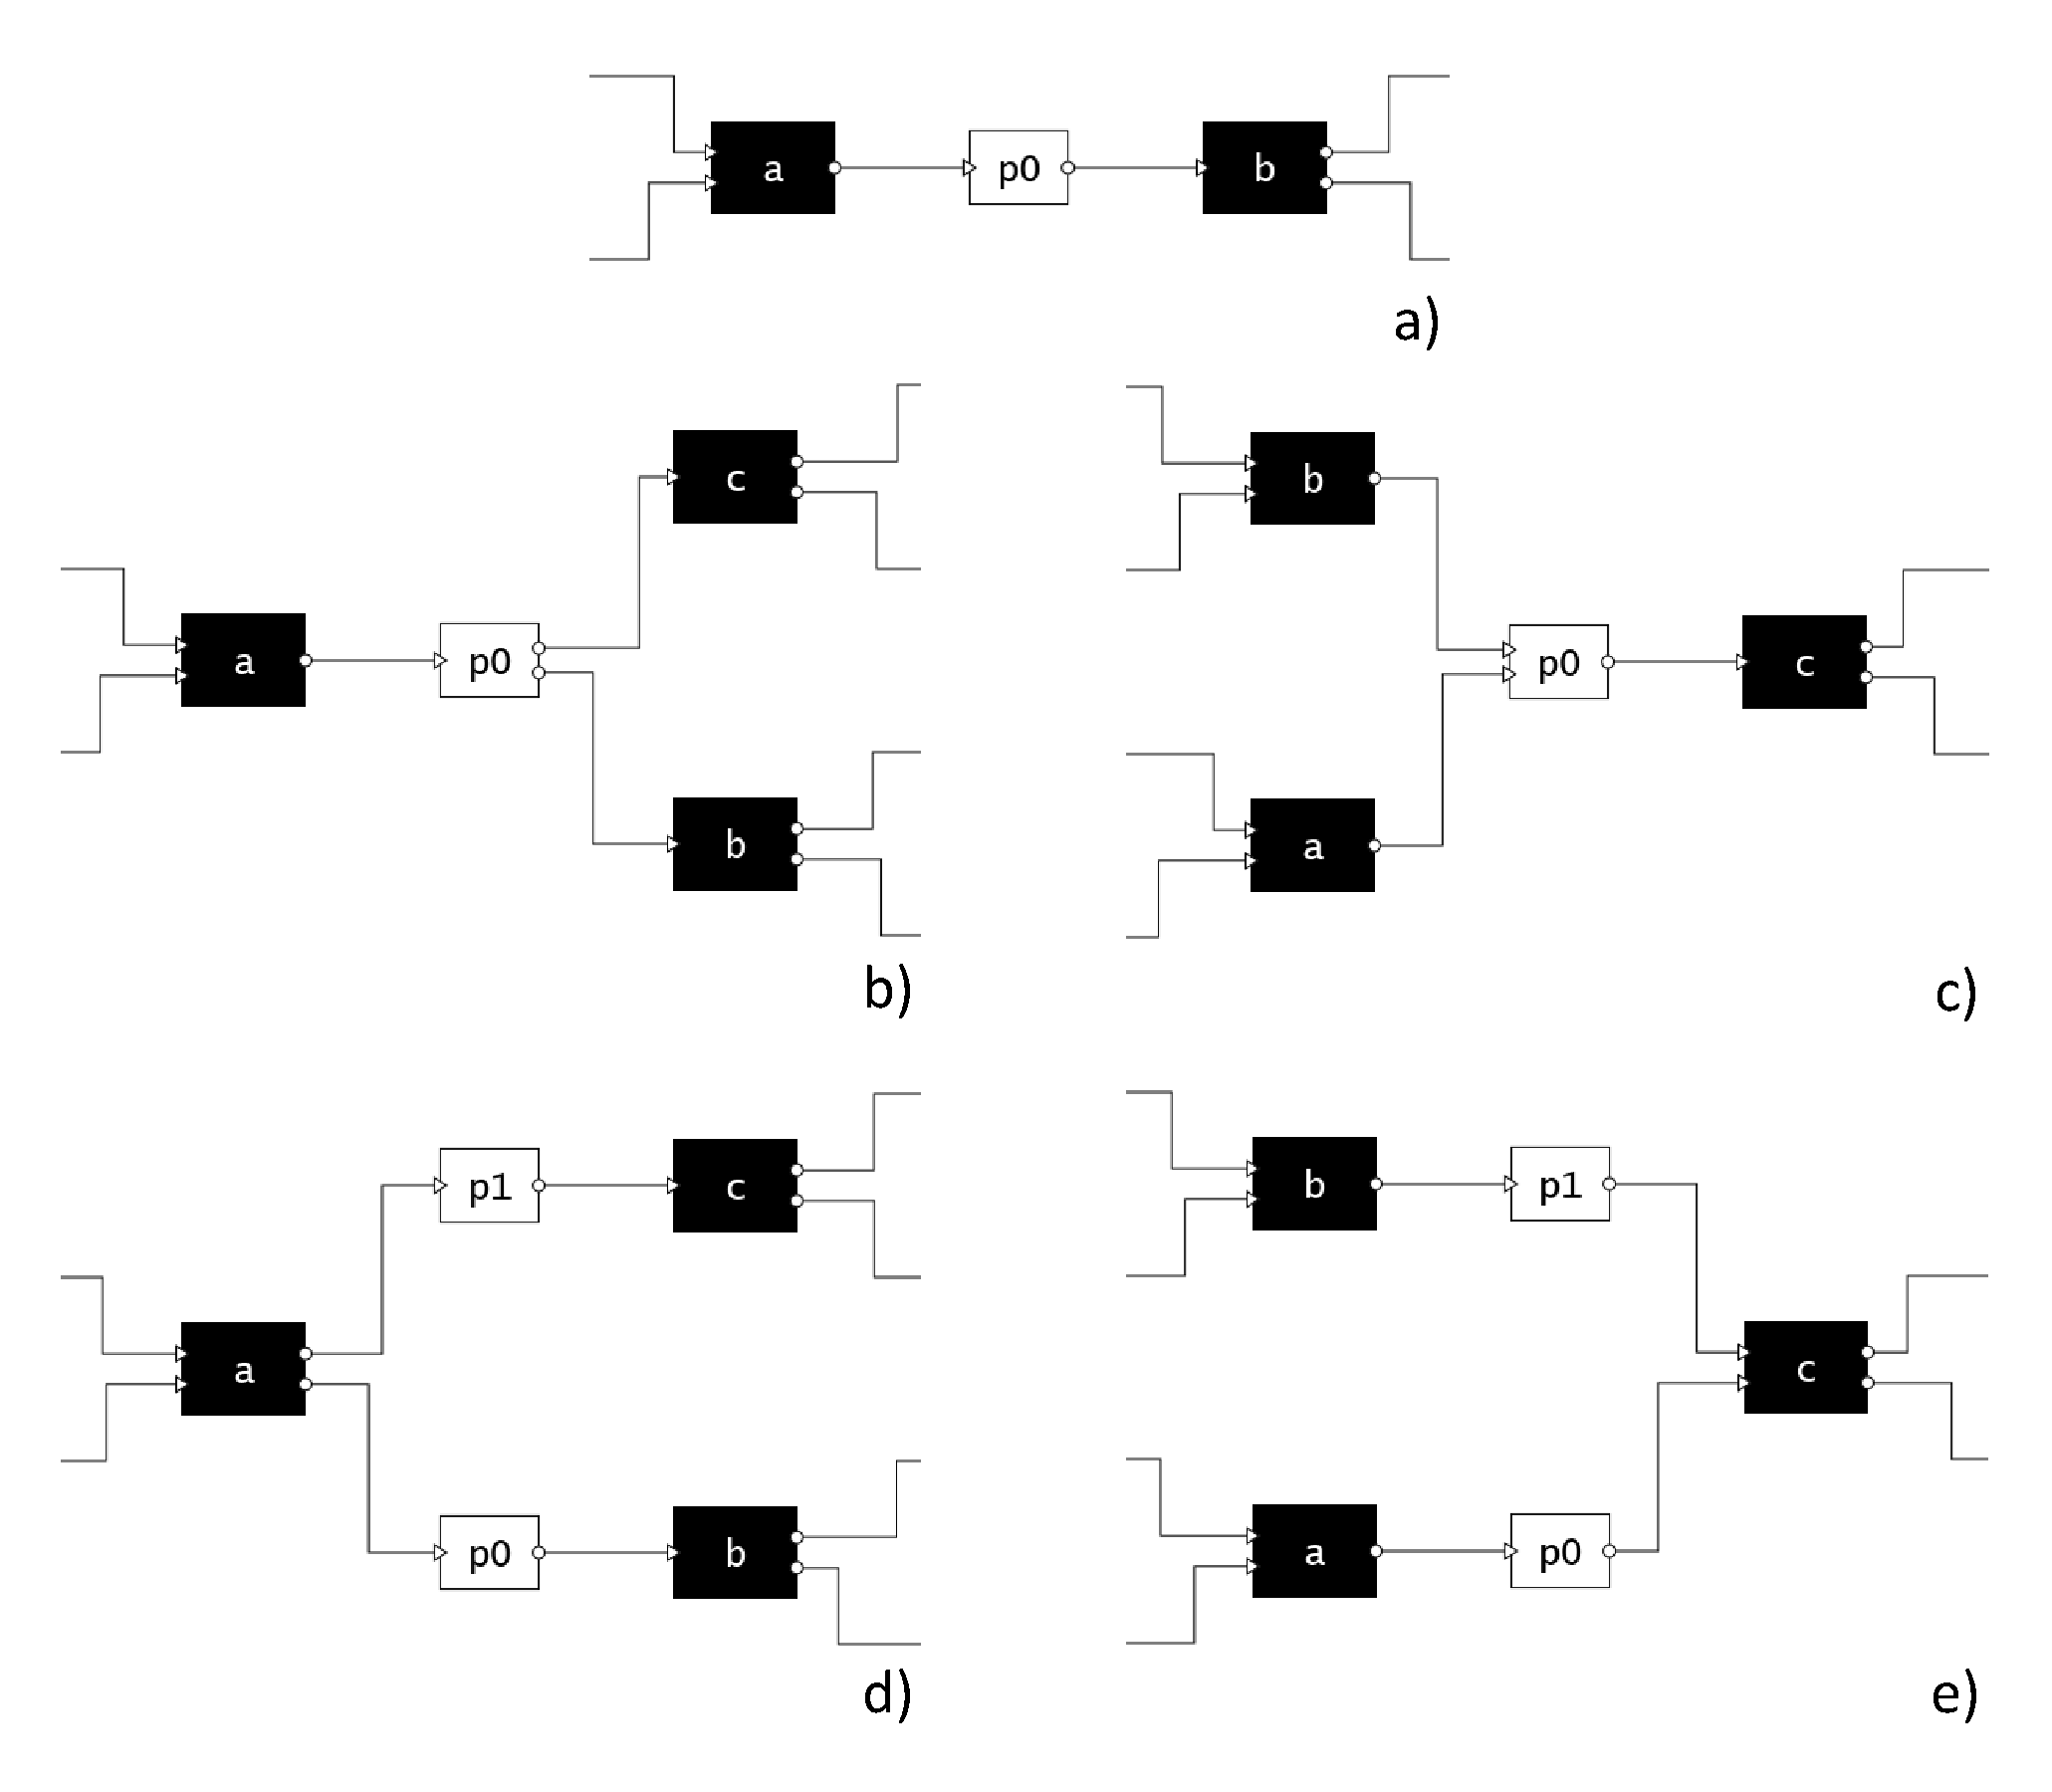
\includegraphics[width=0.8\textwidth]{pics/wfn-patterns.pdf}
\captionstyle{normal}\caption{Process patterns in WFN model. a) Sequence, b) XOR-split, c) XOR-join,\\d) AND-split, e) AND-join.}
\label{fig:wfn-patterns}
\end{figure}

Рассмотрим основные локальные шаблоны протекания процесса, которые можно отобразить с помощью WFN (см. рисунок~\ref{fig:wfn-patterns}).

На рисунке~\ref{fig:wfn-patterns} a) представлена обычная последовательность активностей $a \rightarrow b$.
Данный шаблон предписывает, что после выполнения активности $a$ токен будет помещен в место $p0$.
После этого окажется, что для активности $b$ выполнено условие, что все ее предшественники содержат токены (так как единственный предшественник $b$ это $p0$).
Таким образом, активность $b$ будет выполнена, токен удален из места $p0$ и новые токены будут отправлены по выходным дугам в узлы-последователи активности $b$.
     
На рисунке~\ref{fig:wfn-patterns} b) показан шаблон XOR-split, который реализует выбор одной из активностей после выполнения активности $a$.
После выполнения активности $a$ место $p0$ оказывается занятым токеном, который может быть использован при выполнении только одной из активностей $b$ или $c$.
Таким образом возможно выполнение либо последовательности активностей $a \rightarrow b$, либо последовательности $a \rightarrow c$.

На рисунке~\ref{fig:wfn-patterns} c) показан шаблон XOR-join, который по аналогии реализует выполнение либо последовательности активностей $a \rightarrow c$, либо последовательности активностей $a \rightarrow b$.

На рисунке~\ref{fig:wfn-patterns} d) показан шаблон AND-split, который реализует выполнение обеих активностей $b$ и $c$ после выполнения активности $a$.
Как только активность $a$ оказывается выполненной, то в места $p0$ и $p1$ попадают токены, которые делают возможным выполнение активностей $b$ и $c$.
При этом не важен порядок, в котором эти активности будут выполнены.

На рисунке~\ref{fig:wfn-patterns} e) показан шаблон AND-join, демонстрирующий, каким образом активность $c$ может быть выполнена только после выполнения обеих активностей $a$ и $b$.
Активность $c$ требует для своего выполнения наличия токенов сразу в $p0$ и $p1$, а это может произойти только после выполнения обеих активностей $a$ и $b$.

После описания данной упрощенной модели процесса с помощью WFN можно перейти собственно к алгоритму построения модели на основании журнала событий.
В данном случае журналом событий является просто список сценариев, каждый из которых представляет собой упорядоченную последовательность активностей.
Требуется по предоставленному журналу событий построить модель процесса, описанную с помощью WFN, которая реализует все сценарии из данного журнала.

Будем рассматривать простые сценарии, на которых будет видно, насколько сильно влияют записи журнала событий на реальную модель процесса.
Например, пусть у нас есть идеальная модель некоторого процесса, который состоит из фиксированной последовательности активностей, которые должны быть выполнены в строго определенной последовательности.
Вот эта последовательность активностей: $a \rightarrow b \rightarrow c \rightarrow d \rightarrow e \rightarrow f$.
Данной последовательности активностей соответствует следующая модель процесса, представленная на рисунке~\ref{fig:origin1}

\begin{figure}[h]
\setcaptionmargin{5mm}
%\onelinecaptionsfalse % if the caption is multiline
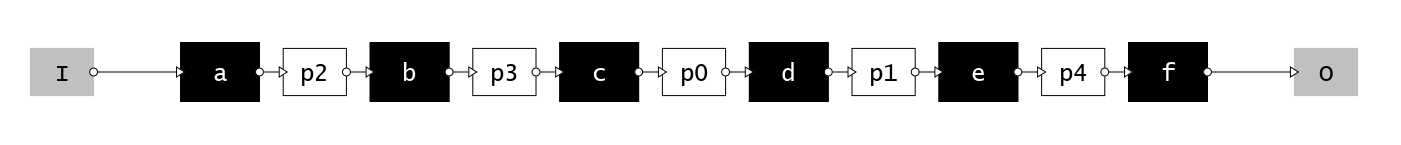
\includegraphics[width=0.95\textwidth]{pics/origin1.png}
\captionstyle{normal}\caption{Модель процесса, построенная по одному сценарию $a \rightarrow b \rightarrow c \rightarrow d \rightarrow e \rightarrow f$.}
\label{fig:origin1}
\end{figure}

Даже если все участники процесса согласны с такой определенной последовательностью активностей, которая необходима для протекания сценария, то обычно в реальности случаются ситуации, когда процесс протекает по-другому.
Представим себе простую ситуацию, когда ввиду спешки или форс-мажора были опущены все промежуточные активности в выполнении сценария и в журнале событий оказалась запись $a \rightarrow f$.
На рисунке~\ref{fig:second1} показана новая модель процесса, которая отражает также и этот появившийся упрощенный сценарий.

\begin{figure}[h]
\setcaptionmargin{5mm}
%\onelinecaptionsfalse % if the caption is multiline
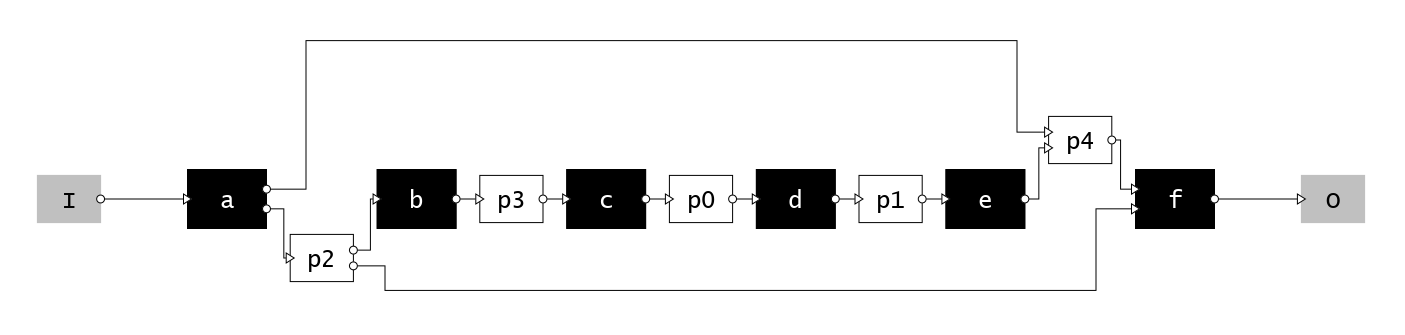
\includegraphics[width=0.95\textwidth]{pics/second1.png}
\captionstyle{normal}\caption{Скорректированная модель процесса после обработки сценария $a \rightarrow f$.}
\label{fig:second1}
\end{figure}

На этом рисунке мы уже видим появление шаблонов XOR-split и XOR-join, и в общем модель процесса заметно усложнилась.

А теперь рассмотрим еще более расширенный журнал событий, в котором попадаются сценарии с другими отклонениями.
В частности рассмотрим сценарий с нарушением порядка выполнения активностей, оборванный сценарий и сценарий с повторным выполнением некоторых последовательностей активностей.
Соберем полный журнал событий, он будет иметь следующий вид:

\begin{eqnarray*}
a \rightarrow b \rightarrow c \rightarrow d \rightarrow e \rightarrow f \\
a \rightarrow f \\
a \rightarrow b \rightarrow d \rightarrow c \rightarrow e \rightarrow f \\
a \rightarrow b \rightarrow c \\
a \rightarrow b \rightarrow c \rightarrow d \rightarrow e \rightarrow b \rightarrow c \rightarrow d \rightarrow e \rightarrow f
\end{eqnarray*}

При построении модели процесса по представленному журналу событий, мы получим схему, изображенную на рисунке~\ref{fig:third1}.

\begin{figure}[h]
\setcaptionmargin{5mm}
%\onelinecaptionsfalse % if the caption is multiline
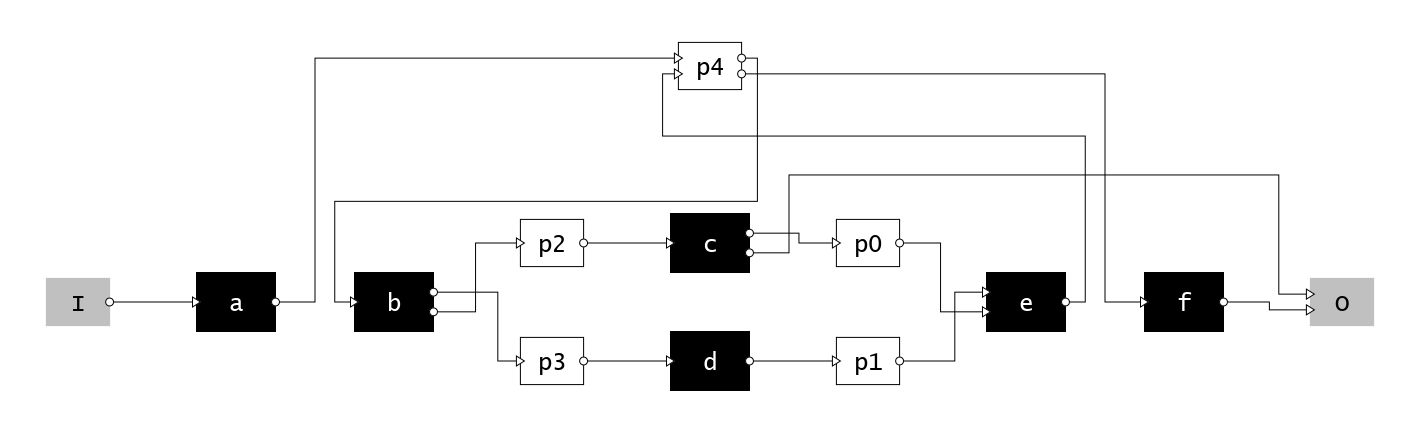
\includegraphics[width=0.95\textwidth]{pics/third1.png}
\captionstyle{normal}\caption{Модель процесса, построенная по журналу событий, содержащему сценарии с искажениями.}
\label{fig:third1}
\end{figure}

Данная модель процесса, конечно, не имеет ничего общего с идеальной моделью с рисунка~\ref{fig:origin1}.
Так же очевидно, что любой анализ следует проводить с использованием этой реальной модели, а не идеальной.
Построение же реальной модели по журналу событий может быть выполнено только автоматически, так как любые искажения реальных сценариев существенно влияют на топологию модели.
Заметим также, что в приведенных примерах показаны совершенно тривиальные сценарии, которые и близко не подходят к сложностям реально протекающих бизнес-процессов.
Поэтому для построения моделей реальных процессов для настоящих журналов событий требуются эффективные алгоритмы.

Опишем простейший алгоритм конструирования модели процесса по журналу событий.
В процессе описания алгоритма будем сразу же показывать его работу на уже рассмотренном модельном журнале событий (обозначим его $L$).

Итак, пусть у нас есть журнал событий

\begin{equation}
\begin{aligned}
L = [
&{a \rightarrow b \rightarrow c \rightarrow d \rightarrow e \rightarrow f},\\
&{a \rightarrow f},\\
&{a \rightarrow b \rightarrow d \rightarrow c \rightarrow e \rightarrow f},\\
&{a \rightarrow b \rightarrow c},\\
&{a \rightarrow b \rightarrow c \rightarrow d \rightarrow e \rightarrow b \rightarrow c \rightarrow d \rightarrow e \rightarrow f}
]
\end{aligned}
\end{equation}

Сначала нужно определить множество всех активностей, присутствующих журнале событий ($A$).
Кроме того, нужно определить множество активностей, с которых начинаются сценарии из журнала событий ($A_I \subset A$), а также активностей, которыми заканчиваются сценарии из журнала событий ($A_O \subset A$).

\begin{equation}
\begin{aligned}
&A = \{a, b, c, d, e, f\} \\
&A_I = \{a\} \\
&A_O = \{c, f\}
\end{aligned}
\end{equation}

Для следующего шага требуется построение матрицы последовательностей активностей ($M_S$).
Данная матрица является квадратной, она имеет размер равный общему количеству активностей, и ее элемент $M_S[x, y]$ содержит единицу, если в журнале событий найдется сценарий, в котором встречается последовательность $x \rightarrow y$.

Матрица $M_S$ для нашего тестового журнала событий выглядит следующим образом:

\begin{equation}
M_S = \begin{vmatrix}
\ & [a] & [b] & [c] & [d] & [e] & [f] \\
[a] & 0 & 1 & 0 & 0 & 0 & 1 \\ 
[b] & 0 & 0 & 1 & 1 & 0 & 0 \\
[c] & 0 & 0 & 0 & 1 & 1 & 0 \\
[d] & 0 & 0 & 1 & 0 & 1 & 0 \\
[e] & 0 & 1 & 0 & 0 & 0 & 1 \\
[f] & 0 & 0 & 0 & 0 & 0 & 0
\end{vmatrix}
\end{equation}

Далее строится матрица отношений $M_R$.
Она имеет такой же размер, что и матрица $M_S$, и ее элементы определяют отношения между активностями, которые должны быть отражены в построенной модели процесса.
Отношение строгого следования между активностями $x$ и $y$ (будем обозначать его через $x \Rightarrow y$) означает, что в журнале событий найдется сценарий, в котором $x \rightarrow y$, но не найдется такого сценария, в котором $y \rightarrow x$.
Другими словами, активности $x$ и $y$ связаны отношением жесткого следования, если $M_S[x, y](1 - M_S[y, x]) = 1$.
Аналогично, активности $x$ и $y$ можно назвать параллельными, если в некоторых сценариях за $x$ может следовать $y$, а в других сценариях за $y$ может следовать $x$.
Условием параллельности активностей является условие $M_S[x, y]M_S[y, x] = 1$ (обозначение $x \ || \ y$).
Если же ни в каких сценариях не обнаружено последовательностей $x \rightarrow y$ или $y \rightarrow x$, то отношение между такими актвностями будем называть неопределенностью.
Условие неопределенности -- $(1 - M_S[x, y])(1 - M_S[y, x]) = 1$ (обозначение $x \ ? \ y$).

Для рассматриваемого журнала событий матрица $M_R$ выглядит следующим образом:

\begin{equation}\label{eqn:r}
M_R = \begin{vmatrix}
\ & [a] & [b] & [c] & [d] & [e] & [f] \\
[a] & ? & \Rightarrow & ? & ? & ? & \Rightarrow \\ 
[b] & \Leftarrow & ? & \Rightarrow & \Rightarrow & \Leftarrow & ? \\
[c] & ? & \Leftarrow & ? & || & \Rightarrow & ? \\
[d] & ? & \Leftarrow & || & ? & \Rightarrow & ? \\
[e] & ? & \Rightarrow & \Leftarrow & \Leftarrow & ? & \Rightarrow \\
[f] & \Leftarrow & ? & ? & ? & \Leftarrow & ?
\end{vmatrix}
\end{equation}

После построения матрицы отношений между активностями можно перейти к построению множества мест для токенов в модели процесса ($P$).
Место для токена должно быть построено для каждой такой пары непересекающихся подмножеств активностей $X \subset A$, $Y \subset A$, что выполнено два условия.
Во-первых, любые две активности из $X$ связаны соотношением неопределенности, также любые две активности из $Y$ связаны соотношением неопределенности.
Во-вторых, любая активность $x \in X$ связана с любой активностью $y \in Y$ соотношением $x \Rightarrow y$. 
В этом случае строится место токена $p(X, Y)$, его узлами-предшественниками становятся все активности из $X$, а узлами-последователями -- все активности из $Y$.

В нашем рассматриваемом случае множество мест токенов выглядит следующим образом:

\begin{equation}
\begin{aligned}
P = \{
& p(\{d\}, \{e\}),
p(\{c\}, \{e\}),
p(\{e\}, \{f\}),
p(\{e\}, \{b\}),
p(\{e\}, \{f, b\}), \\
& p(\{a\}, \{f\}),
p(\{a\}, \{b\}),
p(\{a\}, \{f, b\}),
p(\{e, a\}, \{f\}),
p(\{e, a\}, \{b\}), \\
& p(\{e, a\}, \{f, b\}),
p(\{b\}, \{d\}),
p(\{b\}, \{c\})
\}
\end{aligned}
\end{equation}

Финальным шагом в формировании WFN, который представляет модель процесса, является удаление лишних мест токенов.
Если в наборе мест токенов найдутся два места $p(X, Y) \in P$ и $p(X', Y') \in P$ такие, что $X' \subseteq X$ и $Y' \subseteq Y$, то место $p(X', Y')$ является избыточным, и его можно удалить из модели.

После удаления избыточных мест, финальное множество место токенов примет свой окончательный вид:

\begin{equation}
\begin{aligned}
P = \{
p(\{d\}, \{e\}), p(\{c\}, \{e\}), p(\{e, a\}, \{f, b\}), p(\{b\}, \{d\}), p(\{b\}, \{c\})
\}
\end{aligned}
\end{equation}

Набор приведенных мест токенов приводит нас к модели процесса, изображенной на рисунке~\ref{fig:third1}.

\section{Simple Process Discovery Algorithm Optimization}

В приведенном в предыдущем разделе алгоритме узким местом является конструирование множества мест токенов $P$ с последующим удалением избыточностей.
При возрастании количества сценариев в журнале событий и общего количества активностей количество возможных комбинаций подмножеств активностей для формирования мест токенов растет экспоненциально.
При этом большая часть построенных токенов впоследствии все равно должна быть удалена, так как при построении будет много избыточных мест.
Например, при построенном месте $p(\{a, b\}, \{c, d\})$ в множество $P$ обязательно попадут следующие избыточные места: $p(\{a\}, \{c\})$, $p(\{a\}, \{d\})$, $p(\{b\}, \{c\})$, $p(\{b\}, \{d\})$.
В дальнейшем эти избыточные места будут удалены.
Поэтому требуется подход по построению множества мест токенов $P$, в котором избыточные места отсутствуют с самого начала.

\begin{figure}[h]
\setcaptionmargin{5mm}
%\onelinecaptionsfalse % if the caption is multiline
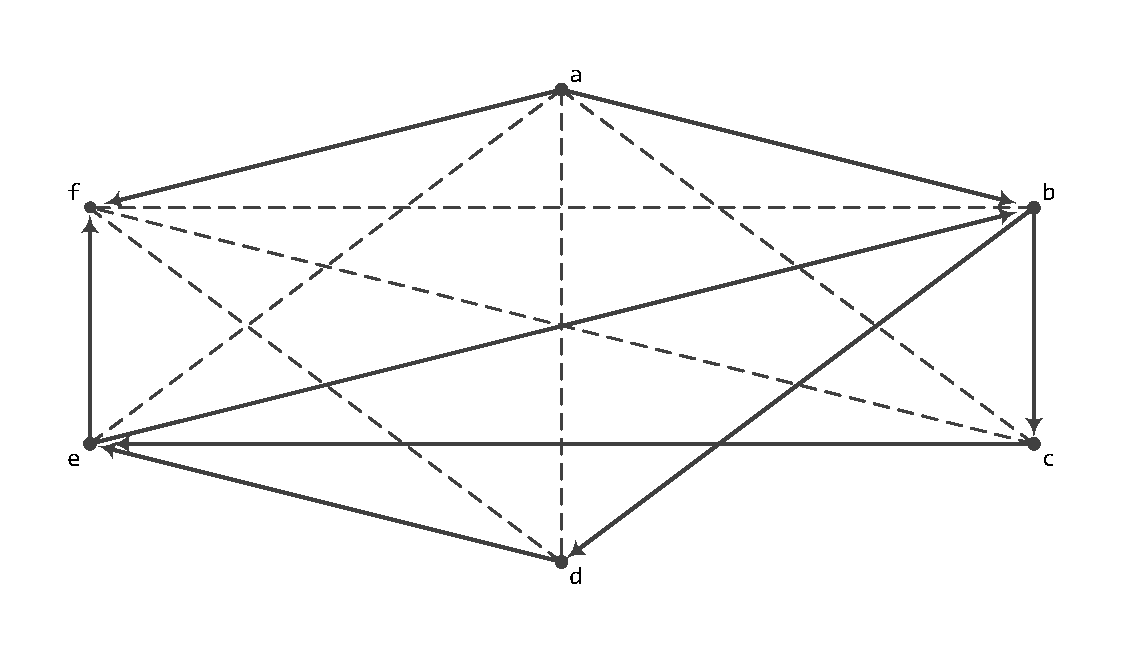
\includegraphics[width=0.8\textwidth]{pics/g_r.pdf}
\captionstyle{normal}\caption{Граф отношение $G_R$. Направленные ребра иллюстрируют отношения строгого следования, пунктирные ненаправленные ребра показывают отношением неопределенности.}
\label{fig:g_r}
\end{figure}

Множество мест токенов без избыточностей может быт построено на основе графа отношений между активностями.
Рассмотрим еще раз матрицу отношений $M_R$ из (\ref{eqn:r}).
В ней нам потребуются только отношения жесткого следования и неопределенности.
Построим вспомогательный граф отношений ($G_R$), узлами которого являются активности.
Далее, рассматриваемый граф содержит ребра двух видов.
Направленные ребра будут отображать отношения жесткого следования (два узла $x$ и $y$ соединены направленным ребром, если $x \Rightarrow y$).
Также в графе будут ненаправленные ребра, соединяющие узлы, связанные отношением неопределенности.
Для нашего рассматриваемого тестового примера граф отношений приведен на рисунке~\ref{fig:g_r}.

После формирования графа отношений $G_R$ нужно провести его стягивание по пунктирным ребрам (которые соответствуют отношению неопределенности).
За один шаг выполняется стягивание по одному ребру по следующим правилам.
Если в графе $G_R$ существует пара активностей $x$, $y$, связанных отношением $x \ ? \ y$, то можно выполнить стягивание по этому ребру.
При этом нужно осуществлять коррекцию отношений с другими активностями графа.
Если в графе есть активность $z$ такая, что $z \Rightarrow x$, $z \Rightarrow y$, то эти отношения удаляются, а вместо них добавляется отношение $z \Rightarrow xy$.
Если в графе есть активность $z$ такая, что $x \Rightarrow z$, $y \Rightarrow z$, то эти отношения удаляются, а вместо них добавляется отношение $xy \Rightarrow z$.
Если в графе есть активность $z$ такая, что $z \ ? \ x$, $z \ ? \ y$, то следует добавить также отношение $z \ ? \ xy$.

\begin{figure}[h]
\setcaptionmargin{5mm}
%\onelinecaptionsfalse % if the caption is multiline
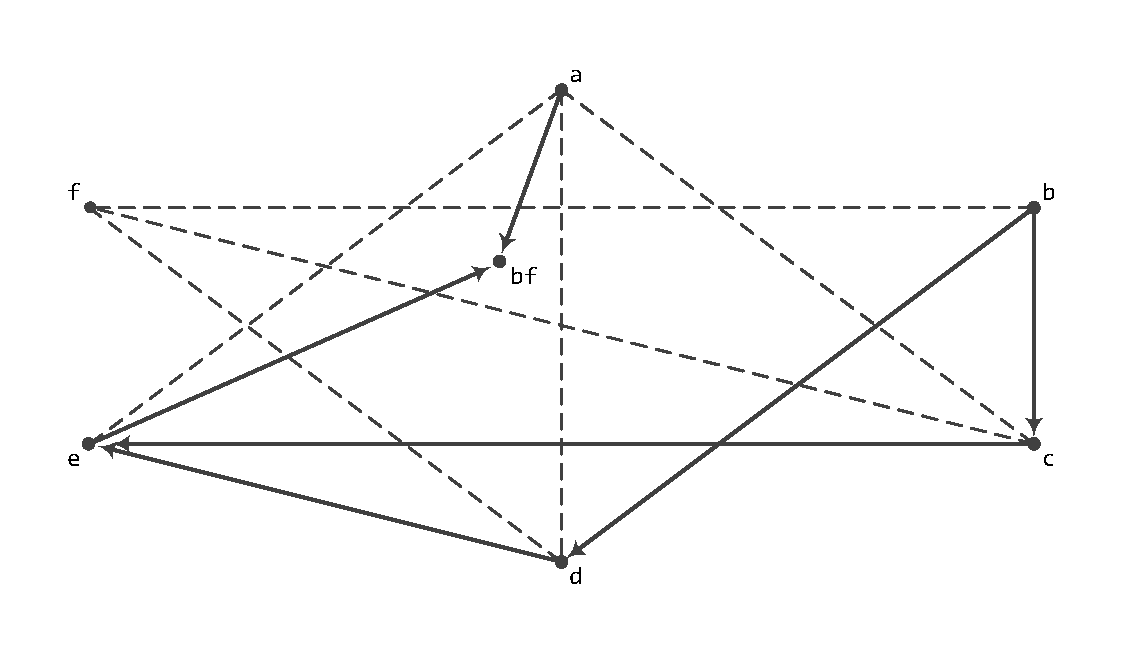
\includegraphics[width=0.8\textwidth]{pics/g_r_reduce1.pdf}
\captionstyle{normal}\caption{Редуцирование графа отношенией активностей. Шаг 1.}
\label{fig:g_r_reduce1}
\end{figure}

\begin{figure}[h]
\setcaptionmargin{5mm}
%\onelinecaptionsfalse % if the caption is multiline
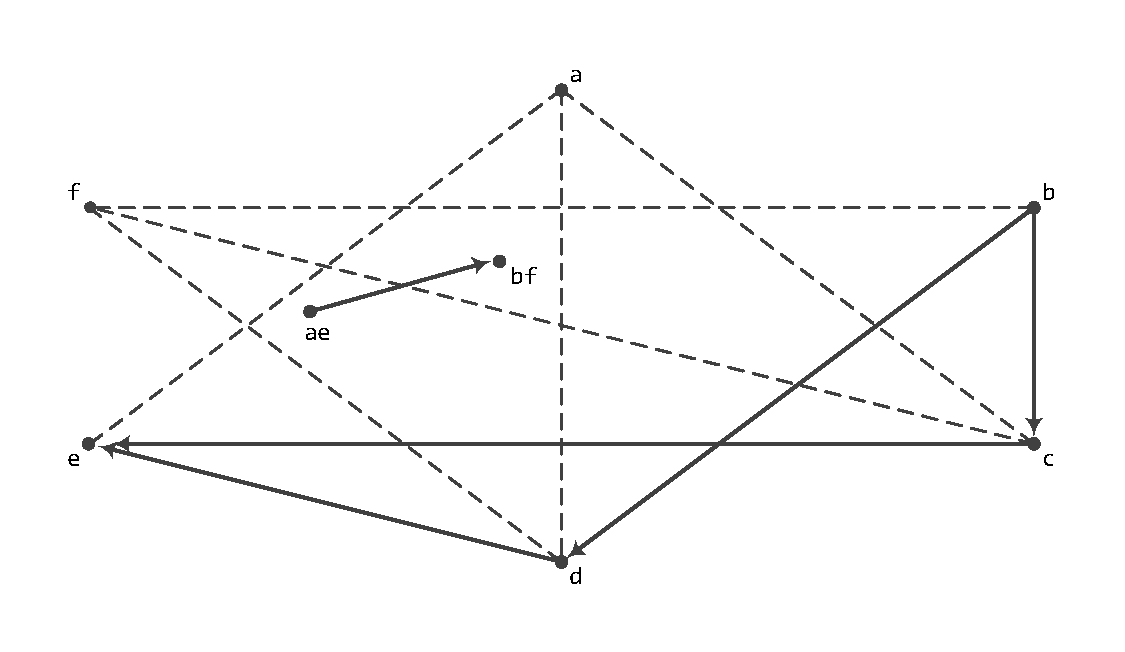
\includegraphics[width=0.8\textwidth]{pics/g_r_reduce2.pdf}
\captionstyle{normal}\caption{Редуцирование графа отношенией активностей. Шаг 2.}
\label{fig:g_r_reduce2}
\end{figure}

На рисунке~\ref{fig:g_r_reduce1} показан один шаг стягивания графа $G_R$ по ребру $b \ ? \ f$.
На рисунке~\ref{fig:g_r_reduce2} показан следующий шаг стягивания графа, уже по ребру $a \ ? \ e$.
Другие стягивания на данном графе выполнять не имеет смысла, после выполнения двух шагов граф содержит 5 направленных ребер, каждое из которых соответствует месту токена в модели процесса, показанной на рисунке~\ref{fig:third1}.

\section{Conclusion}

Conclusion.

\begin{acknowledgments}
The work has been done at the JSCC RAS as part of the state assignment for the topic ... The supercomputer MVS-10P, located at the JSCC RAS, was used for calculations during the research.
\end{acknowledgments}

\begin{thebibliography}{99}

\bibitem{Rettinger}
\refitem{article}
C. Rettinger, C. Godenschwager, S. Eibl, et al., {\it ``Fully Resolved Simulations of Dune Formation in Riverbeds"}, ISC High Performance , LNCS~{\bf 10266}, 3--21 (2017).

\end{thebibliography}

\end{document}
